\documentclass[11pt]{ps_class}

% Required document information
\name         {Isaac Baumann}
\email        {dbaum@uic.edu}
\duedate      {2024-08-01}
\classnum     {ECON 101}
\subject      {Principles of Microeconomics}
\semester     {Fall 2024}
\assignment   {Problem Set 1}
\instructors  {Dr. Johnson}

\begin{document}

This is a general-purpose template for course assignments. It can be used for problem sets, project proposals, research proposals, etc.

\begin{enumerate}
    \item \begin{problem} 
        What is $2+2$? 
    \end{problem}
    
    4

    \item \begin{problem}
        [MWG 1.1] What is the airspeed velocity of an unladen swallow?
    \end{problem}
    
    An African or European swallow?

    \item \begin{problem}
        Do some math
    \end{problem}
    
    $$
    3 + 3 = 6
    $$

    \item \begin{problem}
        Include a figure
    \end{problem}

    \begin{center}
        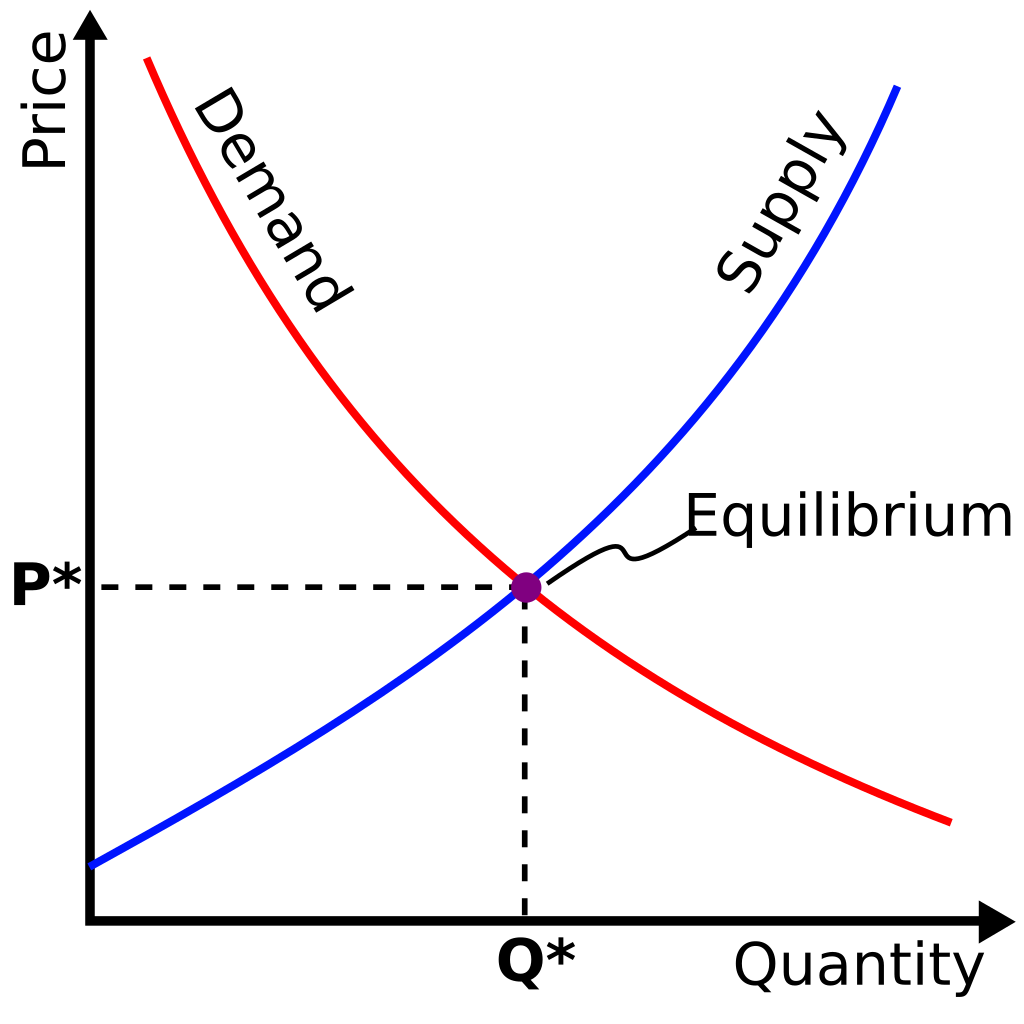
\includegraphics[width=0.25\textwidth]{../figures/supply_demand.png}
    \end{center}
    
\end{enumerate}

\newpage

Some more stuff\footnote{This is a footnote}

\end{document}